\section{Ejercicio 2: Programación Dinámica}
Plantear, implementar con Programación Dinámica el siguiente Problema del Cambio:

Se tiene que dar m centavos de cambio, usando la menor cantidad entre monedas de
denominaciones d1, d2, d3, $\ldots$, dn. Se supone cantidad ilimitada de monedas de cada
denominación. Construir y codificar en Java una solución algorítmica para el problema
que devuelva la cantidad mínima de monedas y sus denominaciones. Analizar el tiempo y
el espacio de ejecución. (Nota: el valor de las monedas no necesariamente es múltiplo
de 5)

\begin{lstlisting}[style=java,caption= Problema del cambio]
  public class ProblemaDelCambio {
    public static void main(String[] args) {
      int [] coinValues = {1,4,6};//lo supongo ordenado
      int n= coinValues.length; 
      int m= 8;
      m++;
      int [][] changeTable = new int[n][m];
      change(changeTable,coinValues,n,m);
    }
  
    public static void change(int [][] changeTable, int [] coinValues,int n, int m){ //m representa m unidades de cambio
  
      for (int i = 0; i < n; i++) {
        changeTable[i][0] = 0;
      }
  
      for (int i = 0; i < n; i++) {
        for (int j = 1; j < m; j++) {
          if(i==0){
            if(j<coinValues[i]){//Caigo fuera de la tabla asi que completa con -1 para indicar que no se puede pagar con las monedas que hay;
              changeTable[i][j] = -1;
            }else{//Asigna j-coinValues[i] osea mueve a la izquierda y a su valor le sumo 1
              changeTable[i][j] = 1 + changeTable[0][(j-coinValues[i])];
            }
          }else if(j<coinValues[i]){//Asigna el valor inmediatamente "arriba" de la tabla
            changeTable[i][j] = changeTable[i-1][j];
          }else if(j>=coinValues[i]){//Asigna el minimo entre ambos
            changeTable[i][j]= Math.min(changeTable[i-1][j], (1 + changeTable[i][(j - coinValues[i])]));
          }
        }
      }
      printChangeTable(changeTable);
      resolve(changeTable, coinValues, n-1, m-1);
    }
  
    public static void printChangeTable(int[][]changeTable){
      for (int i = 0; i < changeTable.length; i++) {
        for (int j = 0; j < changeTable[i].length; j++) {
          System.out.print(changeTable[i][j]+" ");
        }
        System.out.println();
      }
    }
    public static void resolve(int [][]changeTable, int [] coinValues,int i,int j){
      int []solution= new int [coinValues.length];
      while(j>0){//Si no llegamos a la primer columna
        if(changeTable[i][j] == changeTable[i-1][j]){
          i= i-1;//nos desplazamos a la fila de arriba
        }else{
          j = j - coinValues[i];//Nos movemos a la izq
          solution[i]++;//Incrementamos en 1 el indice
        }
      }
  
      System.out.println();
      System.out.println("SOLUCION: ");
      for (int k = 0; k < solution.length; k++) {
        System.out.println(coinValues[k]+"$:"+solution[k]);
      }
    }
\end{lstlisting}

\begin{figure}[!htb]
  \centering
  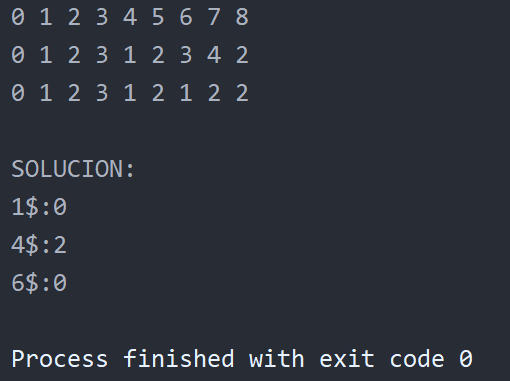
\includegraphics[width=10cm, scale=1]{Images/Punto2/Salida.png}
  \caption{Salida por consola para 8 centavos de cambio y un conjunto de valores de monedas \{1,4,6\}}
\end{figure}

\textbf{Análisis de eficiencia: }Siendo m el valor del cambio y n el numero de monedas entonces en el peor de los casos se tendran m monedas diferentes por lo que el tiempo y el espacio del algoritmo estan en $\Theta(nm)$. Pero al no estar indicado cuales denominaciones forman el cambio, si $C[i,j]=C[i-1,j]$ no se usan monedas $d_i$, en caso contrario se usa una moneda $d_i$ mas las usadas en $C[i,j-d_i]$. Partiendo de $C[n,m]$ hacia $C[0,0]$ haciendo $n-1$ pasos hacia arriba y $C[n,m]$ hacia la izquierda dependiendo cada caso de la denominacion considerada se tendra que el recorrido requiere de un tiempo total de $\Theta(n+C[n,m])$